\documentclass{standalone}
\usepackage{tikz}

\begin{document}
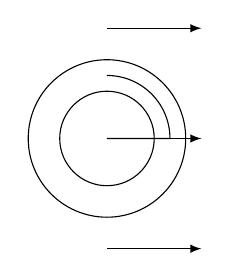
\begin{tikzpicture}[scale=2]
    % Draw the larger circle
    \draw[fill=white] (0,0) circle (0.5);
    
    % Draw the smaller circle inside the larger one
    \draw[fill=white] (0,0) circle (0.3);
    
    % Draw the right angle at the intersection
    \draw (0,0) -- (0:0.4) arc (0:90:0.4) -- (90:0.4) arc (90:0:0.4);
    
    % Draw the arrow pointing to the center of the larger circle
    \draw[-latex] (0,0) -- ++(0:0.6);
    
    % Draw the arrow at the top
    \draw[-latex] (0,0.7) -- ++(0:0.6);
    
    % Draw the arrow at the bottom
    \draw[-latex] (0,-0.7) -- ++(0:0.6);
\end{tikzpicture}
\end{document}